\documentclass[runningheads]{llncs}

\usepackage{amsmath,amssymb,amsfonts}
\usepackage{algorithmic}
\usepackage{graphicx}
\usepackage{textcomp}
\usepackage{xcolor}
\usepackage{float}
\usepackage{url}
\usepackage{caption}

\urldef{\mailsa}\path|mukesh.poudel@usm.edu|
\urldef{\mailsb}\path|nick.rahimi@usm.edu|

\begin{document}

\title{Machine Learning-Based AES Key Recovery via Side-Channel Analysis on the ASCAD Dataset}

\author{Mukesh Poudel\inst{1} \and Nick Rahimi\inst{1}\thanks{Corresponding author}}
\institute{1 School of Computing Science and Computer Engineering, University of Southern Mississippi\\Hattiesburg, MS, USA\\
\email{mukesh.poudel@usm.edu, nick.rahimi@usm.edu}}

\maketitle

\begin{abstract}
    Cryptographic algorithms like Advanced Encryption Standard (AES), Rivest–Shamir–Adleman (RSA) are widely used and they are mathematically robust and almost unbreakable but its implementation on physical devices often leak information through side channels, such as electromagnetic (EM) emissions, potentially compromising said theoretically secure algorithms. This paper investigates the application of machine learning (ML) techniques and Deep Learning models to exploit such leakage for partial key recovery. We use the public ASCAD `fixed' and `variable' key dataset, containing 700-sample and 1400 EM traces respectively from an AES-128 implementation on an 8-bit microcontroller. The problem is framed as a 256-class classification task where we target the output of the first-round S-box operation, which is dependent on a single key byte. We then evaluate standard classifiers (Random Forest (RF), Support Vector Machine (SVM)) and a tailored Convolutional Neural Network (CNN). We also explore the utility of RF-based feature importance for dimensionality reduction. Crucially, we employ this domain-specific Key Rank metric for evaluation, showing its necessity over standard classification accuracy, which remained below 2\% due to low signal-to-noise ratio. Our results show that SVM and RF on full features perform poorly in key ranking. However, RF trained on reduced (top 100) identified via importance analysis achieves Rank 0 (successful key byte recovery) using almost half the attack traces. The implemented CNN as well, despite exhibiting overfitting in terms of validation loss, also achieves Rank 0 efficiently using approximately 65 attack traces for the fixed-key dataset. Thus we conclude that models, particularly CNNs and feature-selected RF, coupled with the Key Rank metric, are an effective tool for side-channel key recovery, confirming the practical vulnerability of the cryptographic implementations.
\end{abstract}

\keywords{Side-Channel Analysis (SCA) \and Machine Learning \and Deep Learning \and AES \and Key Recovery}

\section{Introduction}
Cryptographic algorithms like the Advanced Encryption Standard (AES) are mathematically robust and cannot be compromised through mathematical flaws. However, physical devices executing cryptographic operations lead to unintentional information leakage through various `side channels', such as power consumption, timing variations, and electromagnetic (EM) emissions.\cite{obaid2025enhancing} Electromagnetic analysis (EMA) is a potent form of side-channel analysis (SCA) where attackers non-invasively measure the EM fields radiating from a device during any cryptographic operation. These emissions often contain subtle variations correlated with the intermediate data being processed. And these are often related to the key, which poses a huge challenge. Recent advancements have shown that Machine Learning (ML) and Deep Learning (DL) are powerful tools for automatically learning these complex correlations, potentially outperforming traditional statistical SCA techniques.\cite{berreby2023investigating}\cite{kocher1999differential}

This paper investigates the practical application of ML techniques to recover an AES-128 key byte by analyzing EM side-channel traces from the public ASCAD (ANSSI SCA Database) fixed and variable key dataset\cite{benadjila2020deep}. We frame the problem as a multi-class classification task targeting the output of the first-round AES S-box operation. The low signal-to-noise ratio in the EM traces poses a significant challenge for standard classification metrics like accuracy. This often yields misleadingly poor results. Therefore, a key aspect of this work is the rigorous use of the domain-specific Key Rank metric. Key Rank evaluates an attack's success by determining the position of the true key in a list of all possible key candidates ranked by their likelihood score derived from the ML model's output across multiple traces. This metric directly reflects the practical ability to recover the key, even when per-trace classification accuracy is low.

The contributions of this work are: (1) a comparative performance analysis of standard classifiers (Random Forest (RF), Support Vector Machine (SVM)) and a tailored Convolutional Neural Network (CNN) for AES key byte recovery on the ASCAD dataset, (2) an exploration of RF-based feature importance for dimensionality reduction, its impact on model efficiency and effectiveness, (3) a clear demonstration of the necessity of the Key Rank metric over the standard accuracy for evaluating ML-based SCA success, and (4) confirmation of successful key recovery using both CNN and feature-selected RF models, despite low classification accuracy, highlighting the practical feasibility of ML-based side-channel attacks.

The remainder of this paper is organized as follows: Section 2 details the AES S-box operation, EM leakage principles, the ASCAD dataset, and the specific ML models implemented. Section 3 outlines our experimental setup and the Key Rank evaluation methodology. Section 4 presents and analyzes the results from the RF, SVM, and CNN models. Section 5 discusses the implications of our findings, the accuracy versus Key Rank paradox, and limitations. Finally, Section VI concludes the paper and suggests avenues for future research.

\section{Background and Methodology}
This section provides the necessary background on the target cryptographic operation, the nature of EM side channel leakage, the ASCAD dataset used for experiments, and the specific ML models implemented in our study. We begin with an overview of the AES S-box operation, followed by a discussion of the ASCAD dataset and the data preprocessing steps. We then detail the architectures and hyperparameters for our implemented ML models (Random Forest, SVM, and CNN) and finally reiterate the importance of the Key Rank metric for evaluation. 
\subsection{AES \- Sbox Operation and Leakage }
The Advanced Encryption Standard (AES) is a symmetric block cipher that encrypts data in 16-byte (128-bit) blocks using a key of 128, 192, or 256 bits. AES operates in rounds, with the number of rounds depending on the key size (10 rounds for AES-128, 12 for AES-192, and 14 for AES-256). Each round involves several transformations, including SubBytes, ShiftRows, MixColumns, and AddRoundKey.\cite{huang2025deep} A fundamental non-linear operation within the SubBytes step is the application of the AES S-box substitution, independently to each byte of the internal state. The S-box input for a given byte position $i$ is the result of $\text{Plaintext}[i] \oplus \text{Key}[i]$, where $\oplus$ represents the XOR operation. The S-box then outputs a different byte based on its lookup table:

\begin{equation}
\textit{Sbox\_Output}[i] = \textit{Sbox} (\textit{Plaintext}[i] \oplus \textit{Key}[i])
\end{equation}

\begin{figure}[htbp]
    \centering
    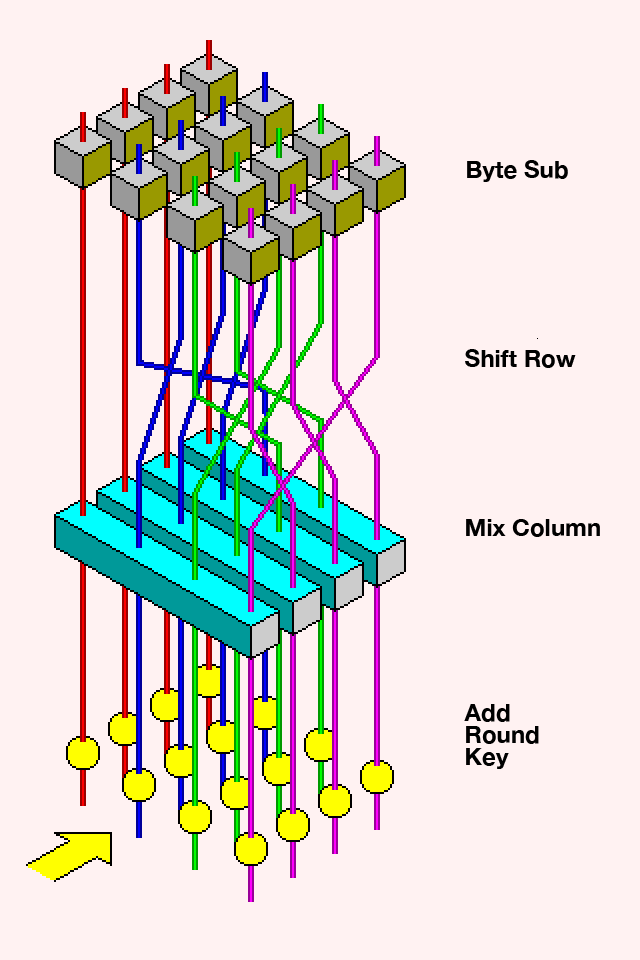
\includegraphics[width=0.3\textwidth,height=0.3\textheight]{fig1Aes.png}
    \caption{Basic Steps of AES Encryption Round (source: \cite{aes_round_commons})}
    \label{fig:aes_steps}
\end{figure}


Figure~\ref{fig:aes_steps} illustrates the four basic steps within each round of AES encryption (excluding the final round which omits MixColumns).

The S-box operation represents a critical point of vulnerability in an AES implementation. Mangard and Schramm identified that although linear operations at the beginning of the S-box do not leak any information, significant leakage occurs in the first masked multiplier where `the XOR gates of this multiplier absorb a different number of transitions for different data inputs.'\cite{mangard2006pinpointing} These differential transitions create a distinctive power consumption pattern that correlates directly with the processed data values and creates the side-channel leakage we aim to exploit. Since the input to the S-box in early rounds (like the first round we target) directly combines known plaintext with the unknown key byte, any leakage related to this operation provides information about the key. 

We adopt the common value-based leakage model, assuming the EM trace contains information correlated with the specific identity (value 0-255) of the $\text{Sbox\_Output}[i]$. Since this output byte depends on both the known $\text{Plaintext}[i]$ and the unknown $\text{Key}[i]$, predicting the S-box output from the trace allows us to deduce $\text{Key}[i]$. As an 8-bit byte can take 256 distinct values, predicting the S-box output becomes a 256-class classification problem. We specifically target the 3rd byte (index $i=2$) in this study.

\subsection{ASCAD Datasets : Fixed-Key (ASCADf) and Variable-Key (ASCADv)}
For this project, we utilize the publicly available ASCAD `fixed-key' dataset, provided by ANSSI.\cite{benadjila2020deep} To further improve the robustness of the algorithm and to mimic a more realistic scenario, we also trained on the 'variable-key' dataset. This dataset presents a more challenging scenario where the secret key changes for each trace in both the profiling and attack sets. We will be referring to the fixed-key dataset as ASCADf and the variable-key dataset as ASCADv throughout this paper for simpler referencing. The ASCAD datasets were chosen for this research due to it being publicly available and well-documented. This is a widely used benchmark in the SCA community and thus helps in reproducible research and comparision amongst existing literatures. 

This particular dataset comprises EM measurements from an AES-128 implementation on an 8-bit ATMega8515 microcontroller, where fixed 128-bit key (for ASCADf) or variable 128-bit keys (for ASCADv) were used. For a supervised Machine Learning problem, this dataset includes precisely labeled data (S-box output for a known key byte ) and corresponding plaintext to help train the classification model. The datasets contains:

\begin{itemize}
    \item \textbf{Profiling Traces:} For ASCADf, A set of 50,000 traces used for training models. Each trace consists of 700 EM measurements (features). For ASCADv, A set of 200,000 traces were used for training and each trace consists of 1400 EM measurements.  Associated metadata includes the plaintext, the fixed key, and pre-calculated labels representing the output of the S-box for the 3rd key byte (index 2).
    \item \textbf{Attack Traces:} A set of 10,000 traces (ASCADf) and 100,000 traces (ASCADv) were used for testing and evaluating the trained models. These traces also contained same number of EM measurements as the profiling counterparts, along with corresponding plaintexts. During the attack phase, the key is treated as unknown.
\end{itemize}


\subsection{Data Preprocessing}

The raw EM traces have different offsets and scales which can impact the performance of Machine Learning models. To fix this, we standardize the training and testing data for both ASCADf (700 traces) and ASCADv (1400 traces) using the mean and standard deviation calculated solely from their respective profiling sets (50,000 traces for ASCADf, and 200,000 traces for ASCADv profiling). This helps make sure that each feature has a zero mean and unit variance. Without scaling, features with higher magnitudes can disproportionately affect the model's decisions, leading to suboptimal performance. Many ML algorithms, particularly those using gradient descent (like CNNs) or distance measures (like SVMs with RBF kernels), perform better and converge faster when input features are on a similar scale and centered around zero. We use Scikit-learn's \textit{StandardScaler} to perform this standardization. We fit the scaler on the training data and then transform both the training and testing data using the fitted scaler. This ensures that the test data is transformed in the same way as the training data, preventing any information leakage from the test set into the model training process.

\subsection{Machine Learning Models}

\textbf{Random Forest (RF):} It is an ensemble learning method that aggregates the predictions of multiple decision trees. We employ Scikit-learn's RandomForestClassifier with $n\_estimators=100$. This provides a good balance between performance and computation. To mitigate overfitting on the high-dimensional data, we apply regularization by setting $max\_depth=20$ to limit the tree complexity and $min\_samples\_leaf=10$ to ensure that each leaf node has sufficient number of samples. Furthermore, RF provides Gini importance scores, which we leverage for feature selection. We train one RF model using all 700 features for ASCADf and 1400 features for ASCADv and another using only the top 100 features as determined by the importance ranking.

\textbf{Support Vector Machine (SVC):} It is a classifier that aims to find an optimal hyperplane to separate different classes. Due to its high computational cost and as it scales poorly with the addition in number of samples and features, we train Scikit-learn's SVC only on the reduced set of 100 features selected by RF. We use the default RBF kernel \textit{(C=1.0, gamma='scale')} and enable probability estimates i.e \textit{probability=True} as it is required for key ranking which relies on the class probability estimates.

\textbf{Convolutional Neural Network (CNN):} We employ a custom CNN architecture implemented in PyTorch, drawing inspiration from ASCAD paper in deep learning-based SCA. The network is designed to learn relevant features directly from the raw EM traces, enabling effective classification of S-box outputs. The architecture details are as follows:
\begin{figure}[hbtp]
    \centering
    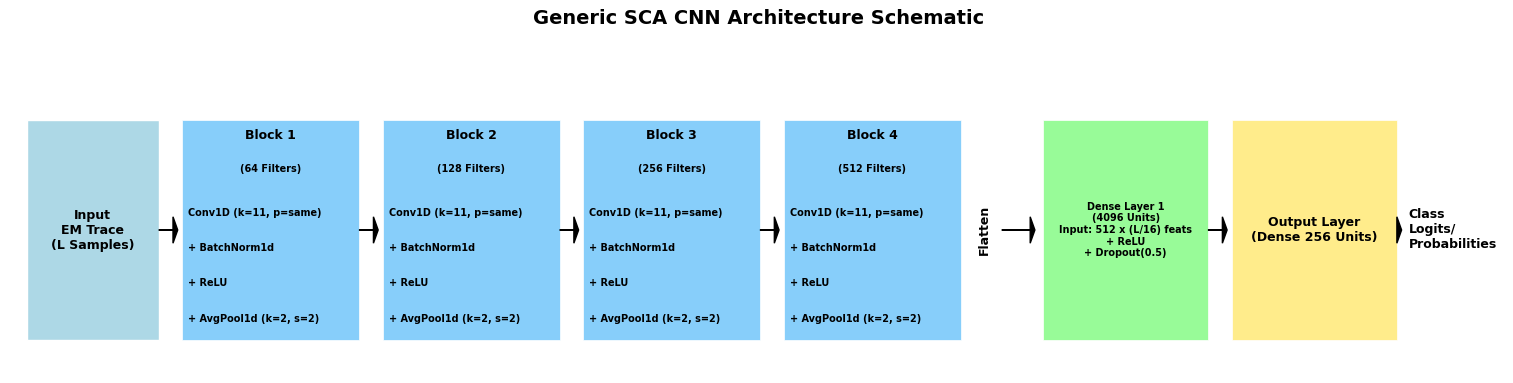
\includegraphics[width=1\textwidth]{Fig2cnnarchitecture.png}
    \caption{CNN Architecture for SCA}
    \label{fig:cnn_architecture}
\end{figure}

\begin{itemize}
    \item \textbf{Input Layer:} Accepts a 1D EM trace (\textbf{700 samples} for ASCADf, \textbf{1400 samples} for ASCADv) as a tensor of shape \texttt{(BatchSize, 1, TraceLength)}
    \item \textbf{Convolutional Blocks (4x):} The network employs four identical convolutional blocks for hierarchical feature extraction. Each block includes:
        \begin{enumerate}
            \item \textit{Conv1d Layer:} Applies 1D convolutions with a kernel size of 11 and padding of 5 (effectively 'same' padding for the convolution operation itself). This choice is directly supported by findings in \cite{benadjila2020deep} which demonstrated that a larger kernel size (e.g., 11) significantly improves SCA-efficiency, especially compared to multiple layers with smaller kernels. The number of output channels (filters) increases progressively: 64, 128, 256, and 512 for the four blocks, respectively, increasing feature map depth to compensate for spatial dimension reduction by pooling layers, allowing the network to learn a richer set of features.
            \item \textit{BatchNorm1d Layer:} Performs batch normalization.
            \item \textit{ReLU Activation:} Applies the Rectified Linear Unit activation function.
            \item \textit{AvgPool1d Layer:} Performs average pooling with a kernel size of 2 and a stride of 2, downsampling the feature map length by a factor of 2 at each block.
        \end{enumerate}
    \item \textbf{Flatten Layer:} Converts the 2D feature maps (channels $\times$ length) from the final pooling layer into a 1D vector. After four pooling layers, an initial trace of length $L$ becomes $L/16$ (with floor operations for odd lengths at intermediate stages).
    \item \textbf{Dense Head (Classification):}
        \begin{enumerate}
            \item \textit{Linear Layer (4096 units):} A fully connected layer with 4096 output units, followed by ReLU activation. The input size to this layer is dependent on the initial trace length:
            \begin{itemize}
                \item For ASCADf (700 input samples, length becomes 43 after pooling): $512 \text{ channels} \times 43 \text{ features} = 22016 \text{ inputs}$.
                \item For ASCADv (1400 input samples, length becomes 87 after pooling): $512 \text{ channels} \times 87 \text{ features} = 44544 \text{ inputs}$.
            \end{itemize}
            \item \textit{Dropout Layer (p=0.5):} Applies dropout regularization.
            \item \textit{Linear Layer (256 units):} A final fully connected layer outputting logits for the 256 possible S-box values.
        \end{enumerate}
    \item \textbf{Training Parameters:}
        \textit{Optimizer} : RMSprop optimizer with a learning rate of $1 \times 10^{-5}$ and a weight decay of $1 \times 10^{-5}$, \textit{Loss Function} : CrossEntropyLoss, \textit{Batch Size} : 100 \textit{Epochs} : 150.
\end{itemize}

The specific CNN architecture is inspired by successful models described in recent literature, and the original ASCAD paper, but has been modified to suit our computational resources and dataset characteristics.

\subsection{Evaluation Metric: Key Rank}
While standard classification accuracy was measured, it proved uninformative due to high noise levels. The primary metric for SCA success is the Key Rank.\cite{picek2019curse} The process is as follows:

\begin{itemize}
    \item Obtain the predicted probability distribution (vector of 256 probabilities) from the trained model for each of the N attack traces. Let P (label=z\textbar trace\_i) be the probability assigned to S-box output value z for trace i.

     \item For each key byte hypothesis k\_guess (from 0 to 255):
        \begin{itemize}
            \item Calculate the hypothetical S-box output \\$\textit{Z\_hyp\_i} = \textit{Sbox}(\textit{$\text{plaintext\_i}$} \oplus \textit {$\text{k\_guess}$})$ for each attack trace $i$ from 1 to $N$.
            \item Calculate the total Summed Log-Probability (SLP) score for this key guess:\\
            $\textit{Score} (\text{k\_guess})=\sum_{i=1}^{N} \log (P (\textit{label}=Z\_hyp\_i | \textit{trace}_i) + \varepsilon)$ \\
            where $\varepsilon$ is a small constant (e.g., 1e-40) to prevent $\log(0)$. The logarithm is used to avoid numerical underflow when multiplying many small probabilities, and to improve computational efficiency by converting multiplications to additions.
        \end{itemize}
    \item Rank the 256 key guesses based on their scores, from highest (most likely) to lowest.

    \item The Rank of the true key byte (k\_true) is its position in this ranked list (Rank 0 indicates it has the highest score and is successfully recovered).

    \item Plotting the Rank vs.\ the number of traces (N) shows the efficiency of the attack. The Key Score Plot (bar chart of Score(k\_guess) vs.\ k\_guess) visually confirms the correct key's dominance.
    
\begin{figure}[htbp]
    \centering
    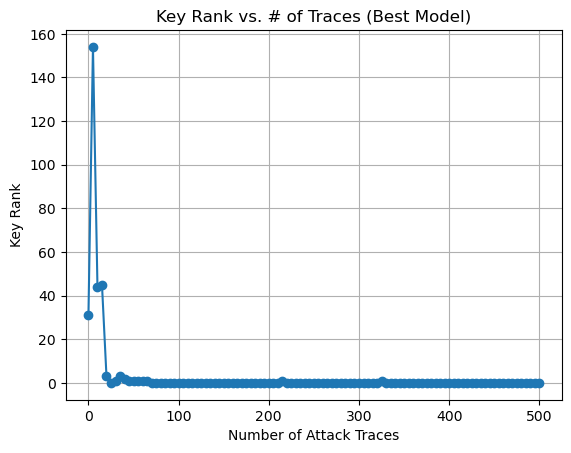
\includegraphics[width=0.5\textwidth]{Fig3keyRankExamplepng.png}
    \caption{Sample Example of a Key Rank Chart}
    \label{fig:key_rank_example}
\end{figure}
Figure \ref{fig:key_rank_example} illustrates a sample Key Rank chart, showing the rank of the true key byte (2) as a function of the number of attack traces used. The graph illustrates how the rank improves with more traces, and successfully recovers the key after ~50 traces.
\end{itemize}
% need to refine and refrence 
The superiority of Key Rank over standard accuracy in this context stems from the nature of SCA. The goal is not to achieve perfect classification of the S-box output for every single noisy trace, which is often an unrealistic expectation due to low signal-to-noise ratio (SNR). Instead, the goal is to distinguish the single correct secret key byte from 255 incorrect hypotheses. Key Rank achieves this by aggregating subtle, consistent evidence (the model's probability assignments) across numerous traces. Even if a model has low accuracy, if it consistently assigns a slightly higher probability to the true S-box output (when the correct key is hypothesized) compared to random outputs, this difference gets amplified when log-probabilities are summed over many traces. This makes the score for the true key dominant, leading to successful recovery, while individual trace noise that confounds accuracy is averaged out.
\section{Experimental Results}
\subsection{Setup}
Experiments were conducted using Python 3.11 with PyTorch (for CNN) and Scikit-learn (for RF, SVM, Scaler) libraries. The Random Forest model utilized 8 cores for parallel processing and 16GB of RAM, while the SVM was limited to a single thread. Training and evaluation were performed on an Nvidia P100 GPU for the CNN model and CPU for RF and SVM models.

\subsection{Random Forest Results}
For the full-feature RF model on ASCADf ($n\_estimators=100$, $max\_depth=20$,$min\_samples\_leaf=10$), 10-fold cross-validation yielded a training accuracy of 43.55\% but a validation accuracy of only 0.46\%. This highlights the challenge of directly classifying individual traces due to the low signal-to-noise ratio inherent in EM leakage. The Key Rank metric is therefore crucial for evaluating SCA success.

In terms of cross-validation, 5 out of 10 folds achieved Rank 0 within 1000 traces. Among these successful folds, the average number of traces required was 492 ($\sigma = 129.21$). The final full-feature RF model exhibited similar performance, requiring hundreds of attack traces to recover the key.

Feature selection using RF's Gini importance significantly improved performance. By training a second RF model on only the top 100 features, the number of attack traces required to achieve Rank 0 was reduced to approximately 200. This represents a 50\% reduction in the number of traces needed for successful key recovery compared to the full-feature model, demonstrating the effectiveness of dimensionality reduction in mitigating overfitting and focusing on the most informative leakage points.

RF on ASCADv with similar parameters and full 1400 features required 750 traces to recover the key. Meanwhile, evaluation on reduced 100 features recovered the key in only 470 traces, reducing the trace count by almost 40\% and re-remphasizing the importance of feature-reduction. 

\begin{figure}[htbp]
    \centering
    \begin{minipage}[b]{0.48\textwidth}
        \centering
        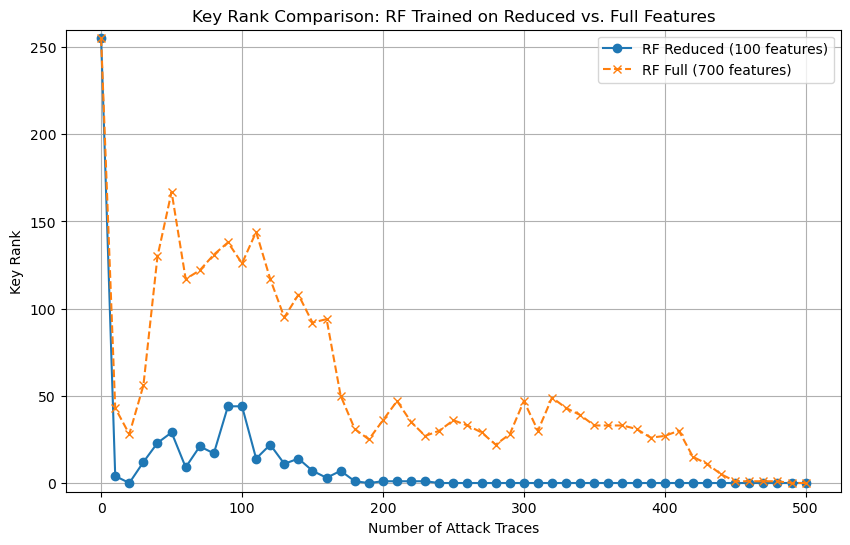
\includegraphics[width=\textwidth]{fig4RandomForrest.png}
    \end{minipage}
    \hfill
    \begin{minipage}[b]{0.48\textwidth}
        \centering
        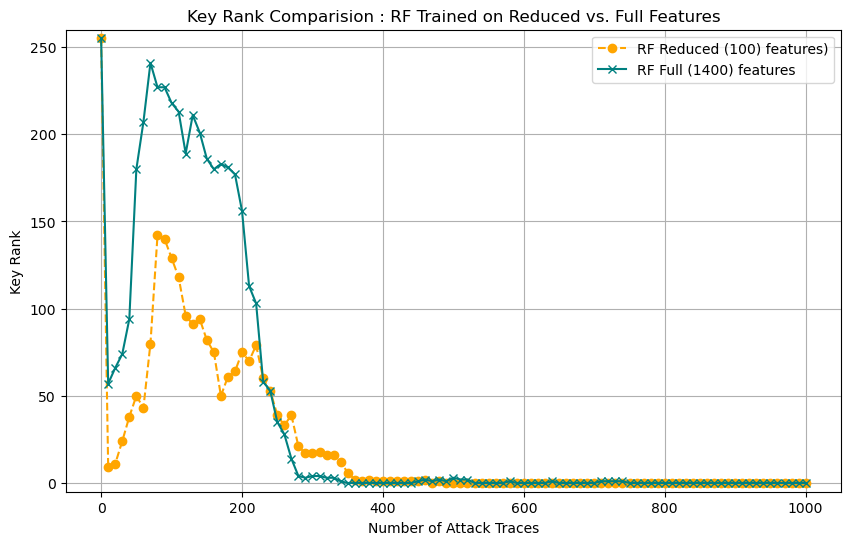
\includegraphics[width=\textwidth]{fig4.1RFASCADv.png}
    \end{minipage}
    \caption{Key Rank Charts for RF on Datasets ASCADf(left) and ASCADv(right)}
    \label{fig:rf_key_rank_combined}
\end{figure}


The feature importance analysis also revealed that leakage is distributed across the trace but with clear concentration in certain time regions. This confirmed the targeted S-box operation leaves electromagnetic fingerprints at specific points in time during execution.


\subsection{CNN Results}
The CNN model exhibited typical deep learning behavior with continuously decreasing training loss (from 5.56 to 5.27) but relatively stable validation loss (around 5.38-5.40), suggesting overfitting by conventional metrics. The final test accuracy was extremely low at only 0.81\%, which would typically indicate a failed model.
\begin{figure}[htbp]
    \centering
    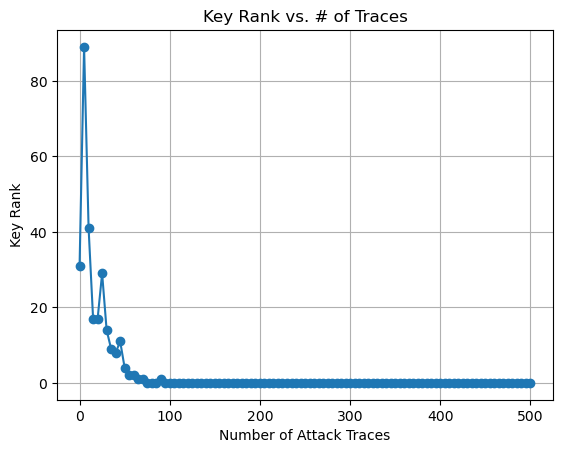
\includegraphics[width=0.5\textwidth]{fig5CNNRank.png}
    \caption{Key Rank Chart for CNN for ASCADf}
    \label{fig:cnn_key_rank}
\end{figure}

However, the key recovery performance told a completely different story. When tested on the attack set, the CNN model's rank of the correct key byte dropped rapidly, reaching Rank 0 consistently after approximately 65 attack traces. This performance was superior to both the full-feature and reduced-feature RF models and is consistent with recent literatures. A reduced learning rate and reduced batch size consistently improved performance. We decided that the current batch size of 100 and learning rate of $1 \times 10^{-5}$ were best in terms of performance and computational efficiency. 

The final key score distribution after using all attack traces showed a clear, dominant peak at the correct key byte 224(for ASCADf), far exceeding the scores of incorrect key guesses. This confirms the CNN successfully learned relevant leakage patterns despite its low classification accuracy.

\subsection{Support Vector Machine Results}
The SVM model was trained only on the reduced set of 100 features selected by RF feature importance, as training on the full 700 and 1400 features would be computationally complex and time consuming. Despite this optimization, the SVM model with RBF kernel for ASCADf required 2392 seconds for training, substantially longer than RF. 

\begin{figure}[htbp]
    \centering
    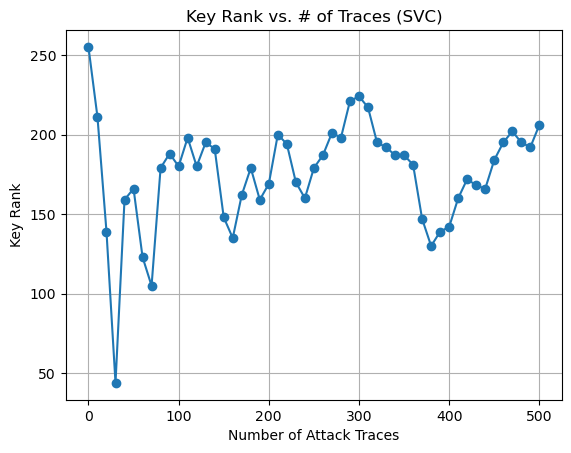
\includegraphics[width=0.5\textwidth]{fig6SVC.png}
    \caption{Key Rank Chart for SVM Model}
    \label{fig:svc_key_rank}
\end{figure}

In terms of key recovery performance, the SVM model failed to recover the key (reach Rank 0) within 500 attack traces. The key rank remained high and fluctuating, suggesting the model was unable to effectively capture the leakage patterns or distinguish the correct key hypothesis from incorrect ones.
\begin{table}[htbp]
    \centering
    \caption{Summary of Model Performance on ASCADf }
    \label{tab:model_comparison}
    \begin{tabular}{|p{2.5cm}|p{1.6cm}|p{2.2cm}|p{2cm}|p{2.6cm}|}
        \hline
        \textbf{Model} & \textbf{Features} & \textbf{Traces to Rank 0} & \textbf{Training Time (s)} & \textbf{Key Recovery} \\
        \hline
        RF (full) & 700 & $\sim$492 & --- & Success \\
        \hline
        RF (reduced) & 100 & $\sim$200 & ---  & Success \\
        \hline
        SVM (reduced) & 100 & $>$500 (failed) & --- & Failure \\
        \hline
        CNN & 700 & $\sim$65 & ---  & Success \\
        \hline
    \end{tabular}
\end{table}

\begin{table}[htbp]
    \centering
    \caption{Summary of Model Performance on ASCADv }
    \label{tab:model_comparison}
    \begin{tabular}{|p{2.5cm}|p{1.6cm}|p{2.2cm}|p{2cm}|p{2.6cm}|}
        \hline
        \textbf{Model} & \textbf{Features} & \textbf{Traces to Rank 0} & \textbf{Training Time (s)} & \textbf{Key Recovery} \\
        \hline
        RF (full) & 1400 & $\sim$750 & --- & Success \\
        \hline
        RF (reduced) & 100 & $\sim$470 & ---  & Success \\
        \hline
        SVM (reduced) & 100 & (in training) & --- & --- \\
        \hline
        CNN & 1400 & (in training) & ---  & --- \\
        \hline
    \end{tabular}
\end{table}
\section{Discussion}
The experiments conducted demonstrate successful AES key recovery from EM leakage using Machine Learning on the ASCAD datasets. The CNN with ASCADf achieved Rank 0 after only 65 traces, while RF for ASCADf with feature selection needed around 200, outperforming SVM. A key finding is that despite low classification accuracy, successful key recovery was possible. RF feature selection has significantly improved performance and proved that focusing on relevant features certainly benefits certain models. RF for ASCADv was able to bring down traces needed from almost 750 to 470, which is almost over 40\% better performance.

One possible explanation for the CNN's superior performance compared to feature-selected RF is that CNNs automatically learn hierarchical and nonlinear features directly from the raw EM traces. This allows CNNs to capture subtle temporal dependencies and complex leakage patterns that manual feature selection may overlook. Additionally, the CNN architecture is designed to be robust against noise by leveraging convolutional filters and pooling operations, which may further enhance its ability to generalize from the noisy data. Thus, while RF with feature selection focuses on the most individually informative features, it might miss intricate interactions present in the full trace data that the CNN is designed to exploit.

While CNNs learn features automatically, RF offers a practical alternative. Overfitting in the CNN (based on validation loss) didn't prevent key recovery, suggesting models can learn generalizable leakage features even while fitting noise. Optimizing for validation loss might not yield the best Key Rank performance. The SVM performed a bit poorly despite using the same reduced feature set as RF. This in turn suggests that ensemble methods like RF might be more robust than kernel methods.

\subsection{Comparison with Existing Literature}
% brief intro then, table compariosion 
The results of this study align with existing literature on ML-based SCA, particularly the effectiveness of CNNs and feature selection techniques. For instance, recent works have shown that CNNs can outperform traditional statistical methods in key recovery tasks, especially when dealing with high-dimensional data like EM traces. The use of RF for feature selection is also consistent with findings that highlight its utility in reducing dimensionality and improving model performance in SCA contexts.
\begin{table}[htbp]
    \centering
    \caption{Comparison with Existing Literature}
    \label{tab:literature_comparison}
    \begin{tabular}{|p{3.5cm}|p{3.5cm}|p{3.5cm}|}
        
        \hline
        \textbf{Reference} & \textbf{Model} & \textbf{Traces to Rank 0} \\
        \hline
        This Study & RF (reduced) & $\sim$200  \\
        \hline
        This Study & CNN & $\sim$65  \\
        \hline
        Huang et al.\cite{huang2025deep} & Inception Net & $\sim$30   \\
        \hline
        Rousselot et al. \cite{rousselot2025scoop} & Scoop - CNN & $\sim$73  \\
        \hline
        Zaid et al. \cite{zaid2020methodology} & CNN & $\sim$191 \\
        
        \hline
    \end{tabular}
\end{table}

\subsection{Potential Countermeasures}
The successful key recovery demonstrates that even standard AES implementations on common microcontrollers are vulnerable to ML-based EM SCA if no specific countermeasures are in place. Potential countermeasures that are commonly used to mitigate such attacks include:
\begin{itemize}
    \item[-]\textbf{Hardware-level:} Noise generation, power supply randomization, specific chip design to reduce EM leakage, shielding.
    \item[-]\textbf{Software-level:} Masking (splitting sensitive values into shares processed independently), shuffling (randomizing the order of operations), or constant-time implementations.
\end{itemize}
These countermeasures aim to reduce the correlation between the EM emissions and the processed data, making it more difficult for attackers to extract sensitive information. However, they often come with trade-offs in terms of performance, complexity, and cost. 

\subsection{Limitations}
The study has its own limitations such as the use of synchronized dataset and the profiling attack methodology, which represents a somewhat best-case scenario for the attacker. While this is very important from a vulnerability and technology standpoint this maynot be a efficient practical implementation in terms of real-world application and penetration. Real-world attacks might face significant timing jitter (desynchronization), increasing complexity. Our profiling attack also assumes known plaintext during the attack phase for key ranking, which may not always be available. The trained models are also specific to the ASCAD dataset and may not generalize well to other datasets or other devices for that matter.

\section{Conclusion}
This work has successfully applied and compared Random Forest, SVM, and Convolutional Neural Network models for AES key recovery via electromagnetic side-channel analysis on the public ASCAD dataset. We demonstrated that despite extremely low classification accuracy, the Key Rank metric revealed successful and efficient key byte recovery using both a tailored CNN and a Random Forest trained on features selected via importance ranking. Our findings confirm that ML techniques can effectively learn subtle leakage patterns, even when models exhibit overfitting by standard validation metrics. Feature reduction using RF importance analysis significantly improved performance, reducing the number of attack traces required for successful key recovery. Deep learning models stood out for their efficiency in learning relevant features directly from raw EM traces. The SVM model, while theoretically powerful, struggled to achieve similar performance, suggesting that ensemble methods like RF may be more robust in this context. The results underscore the practical vulnerability of AES implementations to ML-driven side-channel attacks, highlighting the need for effective countermeasures and robust security evaluation methodologies 

Future work could involve applying these techniques to more challenging scenarios like the desynchronized ASCAD datasets, exploring alternative feature selection methods beyond RF importance, and developing models that can recover multiple key bytes simultaneously to extract the full AES key.\cite{berreby2023investigating} Applying these ML models to datasets from diverse hardware platforms and against AES implementations protected with known countermeasures (e.g., masking) would provide valuable insights into the practical resilience of these defenses. Architecturally, exploring attention mechanisms or residual connections within CNNs could enhance feature learning and potentially improve performance, especially with noisy or desynchronized traces. 

Ultimately, this research highlights the tangible threat posed by ML-driven side-channel attacks, reinforcing the critical need for robust hardware and software countermeasures, alongside rigorous security evaluation methodologies, to protect cryptographic implementations in real-world devices.

\section*{Acknowledgments}
We would like to thank the University of Southern Mississippi for providing the computational resources i.e Magnolia HPC cluster, which was essential for running the experiments and training the models efficiently. 

\bibliography{references}
\bibliographystyle{splncs03_unsrt}


\end{document}
